\section{Technologie abordées}
  \begin{frame}
    \frametitle{Gestion du projet}
    \center
		
\includegraphics[scale=.2]{github-maven.png}
    \begin{block}{Github.com}
      \begin{itemize}
        \item xZwop/R5A
        \item Git, wiki, tickets
      \end{itemize}
    \end{block}

    \begin{block}{Maven}
      \begin{itemize}
        \item[+] Convention, définition des dépendances, gestion du cycle de
          vie.
        \item[-] Convention, définition des dépendances, gestion du cycle de
          vie.
      \end{itemize}
    \end{block}
  \end{frame}

  \begin{frame}
    \frametitle{Technologies abordées}
    \begin{itemize}
      \item Jxta : réseau Pair-à-Pair
      \item Dart
      \item HTML5 + Javascript
      \item GWT
    \end{itemize}
  \end{frame}

  \subsection*{Jxta : réseau Pair-à-Pair}
    \begin{frame}
      \frametitle{Jxta : réseau Pair-à-Pair}
      \begin{itemize}
        \item Technologie open source.
        \item Permettant de faire un réseau	pair-à-pair en Java. 
        \item Le  réseau pair-à-pair est créé sur le réseau existant permettant aux différents noeuds de pouvoir communiquer entre eux.\\
      \end{itemize}
    \end{frame}
    
    \begin{frame}
      \frametitle{Jxta : réseau Pair-à-Pair}
      	\begin{figure}
			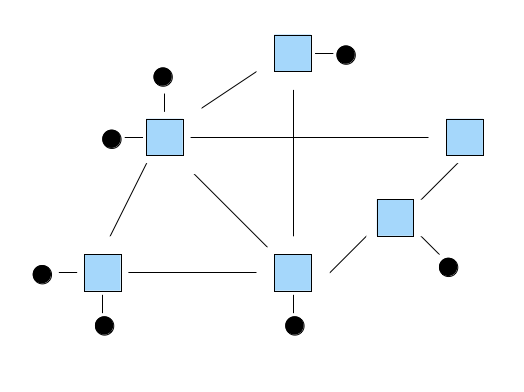
\includegraphics[scale=0.3]{includes/network-model.png}
			\caption{Réseau pair-à-pair}
	   	\end{figure}
    \end{frame}

  \subsection*{Dart}
    \begin{frame}
      \frametitle{Dart}
      \begin{figure}
        \begin{center}
          
\includegraphics[scale=0.4]{includes/dart_logo.png}
        \end{center}
      \end{figure}
      \begin{itemize}
        \item Nouvelle plate-forme
        \item Développé par Google
        \item Langage d'applications Web structurées
        \item Support du multi-tâche (multi-threading)
      \end{itemize}
    \end{frame}
    \begin{frame}
      \frametitle{Dart (suite)}
      \begin{figure}
        \begin{center}
          
\includegraphics[scale=0.4]{includes/dart_logo.png}
        \end{center}
      \end{figure}
      \begin{itemize}
        \item Compilation Javascript
        \begin{itemize}
          \item Exécution dans un navigateur Web
        \end{itemize}
        \item Exécution dans une VM
        \begin{itemize}
          \item Exécution dans un navigateur Web
          \item Exécution sur un serveur
        \end{itemize}
      \end{itemize}
    \end{frame}

  \subsection*{HTML5 + Javascript}
    \begin{frame}
      \frametitle{HTML5 + Javascript}
	  \begin{figure}
		\center
		
\includegraphics[scale=0.40]{html5}
	  \end{figure}
      \begin{itemize}
        \item HyperText Markup Language 5
        \item Nouvelles balises, nouveaux attributs
        \item<2->Web Workers
        \item<3->Server Sent Events
        \item<4->DOM Events
      \end{itemize}
    \end{frame}

  \subsection*{GWT}
    \begin{frame}
      \frametitle{GWT}
      \begin{figure}
		\center
		
\includegraphics[scale=0.60]{gwt-logo}
	  \end{figure}
      \begin{itemize}
        \item Google Web Toolkit
        \item Framework développé par Google
        \item<2->Compatible multi navigateur
        \item<3-> Java vers Javascript
        \item<4->Fonction native 
      \end{itemize}
    \end{frame}

